\chapter{Deskripsi Tugas}
\begin{figure}[H]
    \centering
    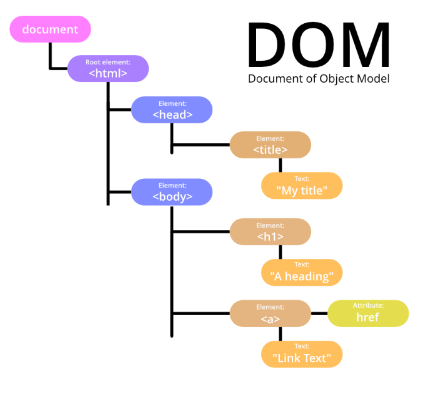
\includegraphics[width=0.7\textwidth]{assets/DomDiagram.png}
    \caption{Struktur Pohon DOM.} \url{https://www.geeksforgeeks.org/java/what-is-document-object-in-java-dom/}
\end{figure}

Document Object Model (DOM) merupakan representasi terstruktur dari dokumen HTML dalam bentuk \textit{tree} yang memungkinkan setiap elemen pada halaman web diakses, dimodifikasi, dan dimanipulasi oleh program. Struktur ini merepresentasikan hubungan antar elemen HTML seperti \textit{parent}, \textit{child}, dan \textit{sibling} sehingga memudahkan pengolahan dokumen secara terprogram.

Struktur sebuah file HTML pada umumnya meliputi elemen \textit{root} \texttt{<html>} yang berisi dua bagian utama yaitu \texttt{<head>} dan \texttt{<body>}. Bagian \texttt{<head>} berisi metadata seperti judul halaman, \textit{link stylesheet}, dan \textit{script}, sedangkan \texttt{<body>} berisi konten utama halaman seperti teks, gambar, tombol, dan elemen HTML lainnya yang ditampilkan kepada pengguna.

Sebuah \textit{website} menampilkan sebuah DOM melalui sebuah file bernama Cascading Style Sheets (CSS) yang bertujuan mendeklarasikan visualisasi elemen-elemen pada pohon. Deklarasi visualisasi ditempelkan pada elemen-elemen yang berkaitan melalui CSS Selector.

Pada Tugas Besar 2 Strategi Algoritma ini, mahasiswa diminta untuk menelusuri dan mencari elemen pada struktur DOM berdasarkan CSS Selector tertentu dengan menggunakan algoritma penelusuran graf yaitu Breadth First Search (BFS) dan Depth First Search (DFS). Algoritma tersebut digunakan untuk menjelajahi struktur pohon DOM guna menemukan elemen yang sesuai dengan \textit{selector} yang diberikan.

Komponen-komponen penting yang terdapat pada tugas besar ini antara lain:

\section{Tags}

\begin{figure}[H]
    \centering
    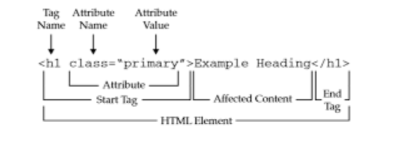
\includegraphics[width=0.7\textwidth]{assets/StrukturHTML.png}
    \caption{Struktur Syntax HTML.} \url{https://tutorial.techaltum.com/htmlTags.html}
\end{figure}

Tag pada HTML merupakan penanda (\textit{markup}) yang digunakan untuk mendefinisikan struktur dan jenis elemen dalam sebuah dokumen HTML. Tag memberi tahu \textit{browser} bagaimana suatu bagian konten harus ditafsirkan dan ditampilkan pada halaman web.

Secara umum, tag HTML ditulis menggunakan tanda kurung sudut (\texttt{< >}). Sebagian besar elemen HTML memiliki pasangan tag pembuka dan tag penutup. Tag pembuka menandai awal suatu elemen, sedangkan tag penutup menandai akhir elemen tersebut. Tag penutup ditulis dengan menambahkan tanda garis miring \texttt{/} sebelum nama tag. Terdapat beberapa jenis tag HTML yang \textit{self-closing}.

Dalam struktur DOM, setiap tag HTML direpresentasikan sebagai \textit{node} pada pohon DOM. Hubungan antar tag membentuk struktur hierarki seperti \textit{parent}, \textit{child}, dan \textit{sibling}. Struktur inilah yang memungkinkan dokumen HTML diproses sebagai sebuah pohon ketika dilakukan penelusuran menggunakan algoritma seperti BFS atau DFS.

\section{CSS Selector}

\begin{figure}[H]
    \centering
    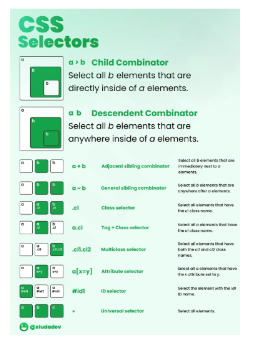
\includegraphics[width=0.7\textwidth]{assets/CSSViz.png}
    \caption{Visualisasi CSS Selector.} \url{https://www.reddit.com/r/webdev/comments/ur6v5m/css_selectors_visually_explained/}
\end{figure}

CSS Selector adalah mekanisme pada CSS untuk memilih elemen HTML tertentu pada struktur DOM agar dapat diberikan aturan \textit{style}. Dengan \textit{selector}, kita dapat menentukan elemen mana yang akan dikenai aturan visual seperti warna, ukuran, atau tata letak. Beberapa \textit{selector} dasar yang umum digunakan adalah sebagai berikut:

\begin{itemize}
    \item \textbf{Tag Selector}\\
    Memilih elemen berdasarkan nama tag HTML. Contoh: \texttt{p} memilih semua elemen \texttt{<p>}.
    
    \item \textbf{Class Selector}\\
    Memilih elemen yang memiliki atribut class tertentu, ditulis dengan tanda titik (\texttt{.}). Contoh: \texttt{.box}
    
    \item \textbf{ID Selector}\\
    Memilih elemen dengan atribut id tertentu, ditulis dengan tanda pagar (\texttt{\#}). Contoh: \texttt{\#header}
    
    \item \textbf{Universal Selector}\\
    Memilih semua elemen HTML. Contoh: \texttt{*}
\end{itemize}

\textit{Combinator} merupakan cara untuk menggabungkan beberapa jenis \textit{selector} dalam penentuan elemen yang akan terpengaruh, dan terdiri dari:
\begin{itemize}
    \item Child Combinator (\texttt{>})
    \item Descendent Combinator (\texttt{" "})
    \item Adjacent Sibling Combinator (\texttt{+})
    \item General Sibling Combinator (\texttt{\textasciitilde})
\end{itemize}

\section{HTML Parsing}
\begin{figure}[H]
    \centering
    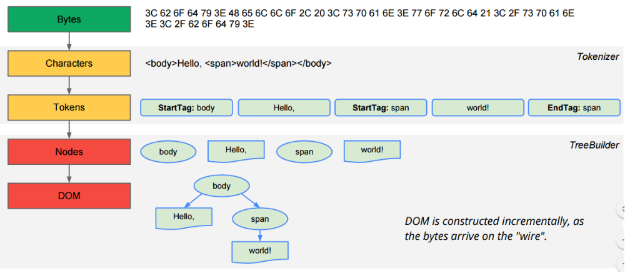
\includegraphics[width=0.7\textwidth]{assets/HTMLParsing.png}
    \caption{Proses Parsing Pohon HTML.} \url{https://stackoverflow.com/questions/3150293/how-does-a-parser-for-example-html-work}
\end{figure}

HTML Parsing adalah proses membaca dokumen HTML dan mengubahnya menjadi struktur data pohon (\textit{tree}) yang merepresentasikan hubungan antar elemen HTML. Pada proses ini, \textit{parser} memproses dokumen HTML secara berurutan, mengenali tag pembuka dan tag penutup, kemudian menyusunnya ke dalam struktur hierarki. 

Setiap tag HTML direpresentasikan sebagai \textit{node} pada pohon. Tag yang berada di dalam tag lain akan menjadi \textit{child node}, sedangkan tag yang membungkusnya menjadi \textit{parent node}. Node paling atas pada struktur ini disebut \textit{root}, yang umumnya merupakan elemen \texttt{<html>}. Dari node \textit{root} tersebut, elemen-elemen lain seperti \texttt{<head>} dan \texttt{<body>} akan menjadi cabang yang membentuk struktur pohon DOM.

Hasil dari proses parsing adalah DOM Tree, yaitu representasi pohon dari dokumen HTML yang memungkinkan elemen-elemen pada halaman web ditelusuri, diakses, dan dimanipulasi secara terstruktur. Struktur pohon ini kemudian dapat digunakan dalam proses penelusuran elemen, misalnya dengan menggunakan algoritma Breadth First Search (BFS) atau Depth First Search (DFS).